\documentclass[10pt, letterpaper]{report}
% !TeX program = xelatex
%==================PREAMBOLO=======================%
\usepackage[utf8]{inputenc}
\usepackage{psvectorian}
\usepackage{pgfplots}
\usepackage[Rejne]{fncychap}
\usepackage[export]{adjustbox}
\usepackage[T1]{fontenc}
\usepackage{lmodern}
\usepackage[shortlabels]{enumitem}
\usepackage{moresize}
\usepackage{graphicx} % Required for inserting images
\usepackage{hyperref}
\usepackage{listings}
\usepackage[table,xcdraw]{xcolor}
\usepackage{amssymb}
\usepackage{amsmath}
\usepackage[italian]{babel}
\usepackage{nicefrac, xfrac}
\usepackage{tikz}
\usepackage{mathrsfs} 
\usepackage{titletoc}
\usepackage{fancyhdr}
\usepackage{psvectorian,lipsum}
\usepackage{fourier-orns}
\usepackage{lipsum}
\usepackage[paper=a4paper,left=25mm,right=25mm,bottom=25mm,top=25mm]{geometry}
\definecolor{light-gray}{gray}{0.95}
\definecolor{cop}{HTML}{f7ecd7}
\definecolor{copAut}{HTML}{ababab}
\definecolor{copAut2}{HTML}{c3c3e6}
\definecolor{purcop}{HTML}{d0d3db}
\definecolor{sapienza}{HTML}{660f1d}
\definecolor{lightSapienza}{HTML}{e3d3d5}
\definecolor{darkgreen}{HTML}{008000}
\definecolor{cartaRiciclata}{HTML}{fcfcf7}
\newcommand{\redText}[1]{\color{red}#1\color{black}}
\newcommand{\code}[1]{\colorbox{light-gray}{\texttt{#1}}}
\newcommand{\codee}[1]{\colorbox{white}{\texttt{#1}}}
\newcommand{\K}{{\mathbb K}}
\newcommand{\notimplies}{%
  \mathrel{{\ooalign{\hidewidth$\not\phantom{=}$\hidewidth\cr$\implies$}}}}
\newcommand{\flowerLine}{ \begin{center}\decofourleft\hphantom{ }\decoone\hphantom{ }\decofourright\hphantom{}\hphantom{aa}
\decofourleft\hphantom{ }\decoone\hphantom{ }\decofourright\hphantom{}\hphantom{aa}
\decofourleft\hphantom{ }\decoone\hphantom{ }\decofourright\hphantom{}\hphantom{aa}
\decofourleft\hphantom{ }\decoone\hphantom{ }\decofourright\hphantom{}\hphantom{aa} 
\decofourleft\hphantom{ }\decoone\hphantom{ }\decofourright\hphantom{}\hphantom{aa}
\decofourleft\hphantom{ }\decoone\hphantom{ }\decofourright\hphantom{}\hphantom{aa}
\decofourleft\hphantom{ }\decoone\hphantom{ }\decofourright\hphantom{}\hphantom{aa}
\decofourleft\hphantom{ }\decoone\hphantom{ }\decofourright\hphantom{}\hphantom{aa}
\decofourleft\hphantom{ }\decoone\hphantom{ }\decofourright\hphantom{}\hphantom{aa}
\end{center}}
\definecolor{g}{RGB}{60, 50, 50}
\newcommand{\textg}[1]{\color{g}{\textbf{#1}}\color{black}}
\newcommand{\teo}[1]{{\large\color{sapienza}\textbf{Teorema #1 :\hphantom{a}}}}
\newcommand{\defi}[1]{{\large\color{sapienza}\textbf{Definizione #1 :\hphantom{a}}}}
\newcommand{\claim}[1]{{\color{sapienza}\textbf{Claim #1 :\hphantom{a}}}}
\newcommand{\lemma}[1]{{\color{sapienza}\textbf{Lemma #1 :\hphantom{a}}}}
\newcommand{\dimo}[1]{{\color{sapienza}\textbf{Dimostrazione #1 :\hphantom{a}}}}
\newcommand{\prop}[1]{{\color{sapienza}\textbf{Proposizione #1 :\hphantom{a}}}}
\newcommand\greybox[1]{%
  \vskip\baselineskip%
  \par\noindent\colorbox{light-gray}{%
    \begin{minipage}{\textwidth}#1\end{minipage}%
  }%
  \vskip\baselineskip%
}
\newcommand\sapbox[1]{%
  \vskip\baselineskip%
  \par\noindent\colorbox{lightSapienza}{%
    \begin{minipage}{\textwidth}#1\end{minipage}%
  }%
  \vskip\baselineskip%
}

\newcommand{\Z}{{\mathbb Z}}
\newcommand{\blank}{{\sqcup}}
\newcommand{\R}{{\mathbb R}}
\newcommand{\N}{{\mathbb N}}
\newcommand{\C}{{\mathbb C}}
\newcommand{\Sn}{{\mathcal S_n}}
\newcommand{\An}{{\mathcal A_n}}
\newcommand{\E}{{\mathcal E}}
\newcommand{\B}{{\mathcal B}}
\newcommand{\mcm}{{\text{mcm}}}
\newcommand{\rg}{{\text{rg}}}
\newcommand{\ve}{{\bar v}}
\newcommand{\spaz}{{\text{\hphantom{aa}}}}
\newcommand{\MCD}{{\text{MCD}}}
\newcommand{\tc}{{\text{ tale che }}}
\newcommand{\supp}{{\text{Supp}}}
\newcommand{\acc}{\\\hphantom{}\\}
\newcommand{\aut}{{\text{Aut}}}
\newcommand{\Span}{{\text{Span}}}
\newcommand{\End}{{\text{End}}}
\newcommand{\cen}{{\text{Centro}}}
\newcommand{\norm}{{\unlhd}}
\newcommand{\ciclS}{{\left \langle }}
\newcommand{\ciclE}{{\right \rangle }}
\newcommand{\boxedMath}[1]{\begin{tabular}{|c|}\hline \texttt{#1} \\ \hline\end{tabular} :}
\newcommand{\shell}[1]{\colorbox{black}{\textcolor{white}{\texttt{#1}}}}
\newcommand{\eqImportante}[1]{\begin{center}\huge\lefthand\hphantom{a}
    \normalsize\texttt{#1}
    \hphantom{aaa}\huge\righthand\end{center}}

\fancyhf{}
\pagestyle{fancy}
\usepackage{pgf-pie}  
\usetikzlibrary{positioning}

\renewcommand{\headrule}{%
\vspace{-8pt}\hrulefill
\raisebox{-2.1pt}{\quad\decothreeleft\decotwo\decothreeright\quad}\hrulefill}

%sta roba serve per il codice C
\definecolor{mGreen}{rgb}{0,0.6,0}
\definecolor{mGray}{rgb}{0.5,0.5,0.5}
\definecolor{mPurple}{rgb}{0.58,0,0.82}
\definecolor{backgroundColour}{rgb}{0.95,0.95,0.92}

\lstdefinestyle{CStyle}{
    backgroundcolor=\color{backgroundColour},   
    commentstyle=\color{mGreen},
    keywordstyle=\color{magenta},
    numberstyle=\tiny\color{mGray},
    stringstyle=\color{mPurple},
    basicstyle=\footnotesize,
    breakatwhitespace=false,         
    breaklines=true,                 
    captionpos=b,                    
    keepspaces=true,                 
    numbers=left,                    
    numbersep=5pt,                  
    showspaces=false,                
    showstringspaces=false,
    showtabs=false,                  
    tabsize=2,
    language=C
}
\lstdefinestyle{CppStyle}{
    backgroundcolor=\color{backgroundColour},   
    commentstyle=\color{mGreen}\ttfamily,
    morecomment=[l][\color{magenta}]{\#}
    keywordstyle=\color{blue}\ttfamily,
    numberstyle=\tiny\color{mGray},
    stringstyle=\color{red}\ttfamily,
    basicstyle=\ttfamily,
    breakatwhitespace=false,         
    breaklines=true,                 
    captionpos=b,                    
    keepspaces=true,                 
    numbers=left,                    
    numbersep=5pt,                  
    showspaces=false,                
    showstringspaces=false,
    showtabs=false,                  
    tabsize=2,
    language=C
}
\lstset{language=C++,
                basicstyle=\ttfamily,
                keywordstyle=\color{blue}\ttfamily,
                stringstyle=\color{red}\ttfamily,
                commentstyle=\color{green}\ttfamily,
                morecomment=[l][\color{magenta}]{\#}
}
%fine roba che serve per il codice C
\usepackage{minted}
\usetikzlibrary{petri}
 %TOGLI COMMENTO SE USI XELATEX
%\usepackage{fontspec}
\title{Ingegneria del Software} %========TITOLO========%
\author{Marco Casu}
\date{\vspace{-5ex}}
\begin{document}

%==================COPERTINA=======================%
\begin{titlepage}
    
\begin{center}
    %TOGLI COMMENTO SE USI XELATEX
   %\setmainfont{Palace Script MT}
   \HUGE Marco Casu\acc
    %\setmainfont{Grand Casino}
     %TOGLI COMMENTO SE USI XELATEX
    %\setmainfont{h Halfroad}
    \HUGE \decothreeleft\hphantom{ }{\HUGE\selectfont Ingegneria del Software}\hphantom{ }\decothreeright
     %TOGLI COMMENTO SE USI XELATEX
   % \setmainfont{Times New Roman}
\end{center}
\thispagestyle{empty}
\begin{figure}[h]
    \centering{
        %l'immagine deve avere una risoluzione 2048x2048
        
\includegraphics[width=1\textwidth ]{images/Copertina.jpg}
    }
\end{figure}
\vfill 
\centering 
\includegraphics[width=0.4\textwidth ]{../../../preamble/Stemma_sapienza.png} \acc
\centering \Large \color{sapienza}Facoltà di Ingegneria dell'Informazione,
Informatica e Statistica\\
Dipartimento di Informatica
\end{titlepage}

%===================FINE COPERTINA======================%
\newpage
\pagecolor{cartaRiciclata}%\setmainfont{Algerian}
\Large
Questo documento è distribuito sotto la licenza 
\color{blue}\href{https://www.gnu.org/licenses/fdl-1.3.txt}{GNU}\color{black},  
è un resoconto degli appunti (eventualmente integrati con libri di testo) tratti dalle lezioni del corso di Ingegneria del Software
\hphantom{a}per la laurea 
triennale in Informatica. Se dovessi notare errori, ti prego di segnalarmeli.
\vfill
\begin{figure}[h!]
    \raggedright
    
\includegraphics[width=0.4\textwidth,right ]{../../../preamble/tomodachi.pdf} 
\end{figure}
\newpage %\setmainfont{Times New Roman}
\normalsize
\tableofcontents 
\newpage

%==================FOOTER e HEADER=======================%
\fancyhf{}
\fancyhead[L]{\nouppercase{\leftmark}}
\fancyhead[R]{Sezione \thesection}
\fancyfoot[C]{\thepage}
\fancyfoot[L]{Appunti di Ingegneria del Software}
\fancyfoot[R]{ Marco Casu}
%\fancyfoot[R]{\setmainfont{Palace Script MT}\huge Marco Casu \setmainfont{Times New Roman}}
%==================FOOTER e HEADER=======================%

%Ricorda del comando \flowerLine per separare le sottosezioni. Le sezioni si separano nelle diverse pagine

%==================INIZIO======================%
\chapter{Introduzione}
Quando si vuole produrre software complesso, non terminante e di grandi dimensioni, è 
necessario ingegnerizzare il metodo di sviluppo ed astrarre il modello del software. 
L'obiettivo dell'ingegneria del software non riguarda il codice stesso, ma la definizione 
dell'architettura e delle specifiche del sistema. Vanno definiti i processi di sviluppo.\acc 
È cruciale l'analisi dei requisiti, e la modellizazzione delle specifiche di sistema, UML è un 
linguaggio che permette di descrivere la \textit{dinamica} ed il comportamento del modello. Una volta 
definiti i requisiti, si affronta la fase di \textit{planning}.\acc 
Un modello computazionale che risulterà utile prende il nome di \textit{digital twin}, ossia 
una copia del software sulla quale è possibile testare i vari \textit{scenari operativi}, tramite la 
generazione di test automatici. Essendo il sistema discreto, a stati non necessariamente 
finiti, è possibile descriverlo tramite una catena di Markov. \acc 
Nella produzione software prendono parte 3 principali attori\begin{center}
    \includegraphics[width=0.4\textwidth ]{images/attori.eps}
\end{center}
\section{Modellazione}
Il linguaggio UML è utilizzato per modellare sia i requisiti che il sistema stesso, 
esso è composto da differenti diagrammi\begin{itemize}
    \item activity 
    \item use case 
    \item sequence 
    \item class 
    \item state 
    \item context
\end{itemize}
Si consideri il seguente esempio di un sistema di gestione di una clinica psichiatrica, 
lo schema in figura \ref{clinica}, è il context diagram, e rappresenta l'insieme dei serivizi che il 
sistema offre.
\begin{figure}[h!]
    \centering 
    \includegraphics[width=0.7\textwidth ]{images/context.eps}
    \caption{context diagram}
    \label{clinica}
\end{figure}
Un activity diagram descrive l'evoluzione di una certa attività/task che il sistema 
deve poter implementare, si considere l'esempio in figura \ref{activity} riguardante 
l'inserimento di un paziente nella clinica.
\begin{figure}[h!]
    \centering 
    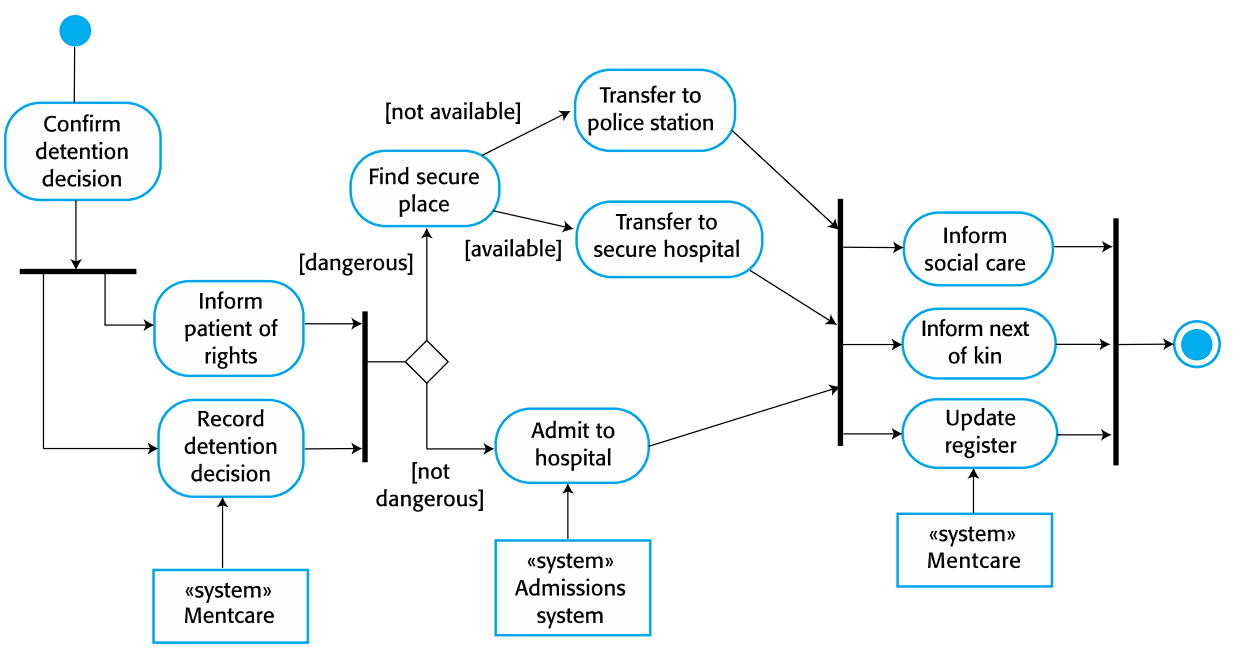
\includegraphics[width=0.7\textwidth ]{images/acrivity.png}
    \caption{activity diagram}
    \label{activity}
\end{figure}
\chapter{Planning del Progetto}
Il planning di un progetto, consiste nel suddividere il carico di lavoro in diverse 
parti, da assegnare ai vari membri del team, cercando di prevedere possibili problemi 
che potrebbero insorgere durante lo sviluppo, pensando e preparando eventuali modi per 
risolverli.\acc 
Il \textit{piano del progetto} viene preparato all'inizio dei lavori, viene utilizzato per 
comunicare ai vari membri del team ed al cliente come esso è stato suddiviso. Le fasi in cui 
il planning viene definito sono \begin{itemize}
    \item Durante la proposta, quando avviene la contrattazione con il cliente riguardo lo sviluppo del 
    software 
    \item Durante la fase di avvio dei lavori, quando si decide come e a chi assegnare il lavoro, e 
    quali risorse dovranno essere allocate 
    \item Periodicamente durante lo sviluppo, monitorando ed appositamente modificando i piani in base 
    all'andamento del progetto e alle esperienze pregresse
\end{itemize}
Lo scopo del planning è quello di avere un idea chiara sul progetto in modo che si possa decidere 
un prezzo d'accordo con il cliente, valutando e stimando quanto denaro sarà necessario per 
lo sviluppo considerando variabili del tipo \begin{itemize}
    \item costo dei dipendenti 
    \item costo dell'hardware necessario 
    \item costo del software
\end{itemize}
Durante la fase di planning, sono noti i requisiti del sistema, ma non è ancora chiara la 
struttura del software, tanto meno la sua implementazione, il planning deve essere 
preciso a sufficienza per far si che sia possibile definire il budget e lo staff necessario. 
Inoltre bisogna definire i meccanismi con la quale verrà monitorato lo sviluppo.
\flowerLine
\section{Sviluppo Plan-Driven}
Con \textit{plan driven development}, si intende un approccio all'ingegneria del software in cui 
i processi di sviluppo sono programmati in principio, in maniera dettagliata. Si basa sulle tecniche di 
gestione, tipiche dei progetti ingegneristici, e sulle tecniche "classiche" di gestione di grandi 
progetti software.\acc 
Un project plan ha l'obiettivo di definire e monitorare il lavoro da svolgere, in che modo 
deve essere svolto, da chi, e quali prodotti sono necessari. È scopo del manager, servirsi di un project 
plan (che da ora chiameremo semplicemente "piano") 
per supportare le decisioni da prendere durante lo sviluppo, e per misurarne il progresso.\begin{itemize}
    \item Un lato favorevole di tale approccio, è che una pianificazione a monte permette di 
    aggirare problemi organizzativi in principio, determinando potenziali problemi e dipendenze 
    da soddisfare prima che il progetto sia avviato, piuttosto che durante la lavorazione. \begin{quote}
        \textit{meglio prevenire che curare}
    \end{quote}
    \item Un lato sfavorevole, è che molte decisioni prese in principio vanno riviste dati possibili 
    cambiamenti dell'ambiente in cui il software deve essere adoperato.
\end{itemize}
Un piano deve definire, le risorse disponibili per il progetto, la suddivisione 
del carico di lavoro, una schedule per portare a termine il lavoro. Precisamente, un piano consiste 
nelle seguenti sezioni\begin{enumerate}
    \item introduzione 
    \item organizzazione del progetto 
    \item analisi dei rischi 
    \item risorse hardware e software necessarie 
    \item struttura di scomposizione del lavoro
    \item schedule del progetto 
    \item meccanismi di monitoraggio e report
\end{enumerate}
Ci sono inoltre altri tipi di "piano" che possono essere aggiunti a quello principale come supporto:
\begin{center}
    \begin{tabular}{cc}
        \rowcolor[HTML]{9698ED} 
        Piano                                           & Descrizione                                                                                                                                                                                                                                                              \\
                                                        &                                                                                                                                                                                                                                                                          \\
        \rowcolor[HTML]{DAE8FC} 
        \textbf{Configuration managment plan}           & \begin{tabular}[c]{@{}c@{}}descrive la configurazione delle \\ procedure di gestione, la loro \\ struttura ed il loro utilizzo\end{tabular}                                                                                                                              \\
        \rowcolor[HTML]{ECF4FF} 
        {\color[HTML]{000000} \textbf{Deployment plan}} & {\color[HTML]{000000} \begin{tabular}[c]{@{}c@{}}descrive come il software deve \\ essere integrato con l'apposito \\ hardware di riferimento del cliente, \\ con eventuali piani di migrazione dei \\ dati in uso su sistemi precedentemente \\ adoperati\end{tabular}} \\
        \rowcolor[HTML]{DAE8FC} 
        \textbf{Maintenance plan}                       & \begin{tabular}[c]{@{}c@{}}predizione dei requisiti, costi e lavoro \\ per la manutenzione del software\end{tabular}                                                                                                                                                     \\
        \rowcolor[HTML]{ECF4FF} 
        {\color[HTML]{000000} \textbf{Quality plan}}    & {\color[HTML]{000000} \begin{tabular}[c]{@{}c@{}}descrizione delle procedure e standard di \\ qualità utilizzati nel progetto\end{tabular}}                                                                                                                              \\
        \rowcolor[HTML]{DAE8FC} 
        \textbf{Validation plan}                        & \begin{tabular}[c]{@{}c@{}}descrizione degli approcci, risorse e schedule \\ utilizzati per la convalida del sistema\end{tabular}                                                                                                                                       
        \end{tabular}
\end{center}
Il planning del progetto è un processo \textit{iterativo} che viene sottoposto 
ad inevitabili cambiamenti durante lo sviluppo progressivo. Con l'aumentare delle informazioni 
relative al sistema durante lo sviluppo, è doveroso revisionare i requisiti iniziali,  
dei cambiamenti nel business possono portare a grandi cambiamenti nei requisiti del progetto, portando 
ad un eventuale ri-pianificazione totale.
\subsubsection{Assuzioni del planning}\begin{itemize}
    \item Le assunzioni da fare durante la definizione del project plan 
    non devono essere ottimistiche, bensì 
    realistiche.
    \item Durante lo sviluppo insorgeranno inevitabilmente dei problemi che causeranno dei ritardi 
    nella consegna. 
    \item Le assunzioni iniziali e lo scheduling saranno inevitabilmente soggetti a problemi inaspettati.
    \item Bisogna sempre considerare ogni imprevisto, in modo che eventuali problemi non 
    siano troppo gravanti sulla schedule.
\end{itemize}\begin{center}
\begin{figure}[h!]
    \centering 
    \includegraphics[width=1\textwidth ]{images/projectPlanning.eps}
    \caption{Processi del project planning}
\end{figure}\end{center}
In caso di seri problemi durante lo sviluppo, è necessario applicare delle procedure di 
\textit{mitigazione del rischio}, onde evitare il fallimento del progetto. In congiunzione a ciò, 
può essere necessaria la ripianificazione del progetto.\\ 
Ciò può comportare la rinegoziazione con il cliente dei risultati attesi 
e dei vincoli da rispettare. Una nuova schedule, e data di consegna dovrà essere definita in modo 
da stabilire un accordo con il cliente.
\flowerLine 
\section{Scheduling del Progetto}
\defi{} : Con \textit{scheduling del progetto} si intende il processo di decisione riguardante 
il come il carico di lavoro di un progetto deve essere organizzato in differenti attività, ed 
in che ordine queste attività devono essere eseguite.\acc 
Viene stimato un calendario con i tempi necessari al completamento delle attività, lo sforzo 
necessario ed il personale al quale delegarlo. È anche necessaria una stima delle risorse 
necessarie, come lo spazio su disco necessario per il software, ed il budget da 
muovere.\begin{enumerate}
    \item Suddivisione del progetto in varie attività e stima delle risorse per ognuna di esse 
    \item Organizzazione delle attività da eseguire in concorrenza per ottimizzare i tempi 
    \item Minimizzazione delle dipendenze fra le varie attività, in modo da ridurre i 
    ritardi dovuti ad attese 
\end{enumerate}
Questi ultimi fattori dipendono anche dall'intuizione e dalla esperienza del project manager.
\begin{center}
    \begin{figure}[h!]
        \centering 
        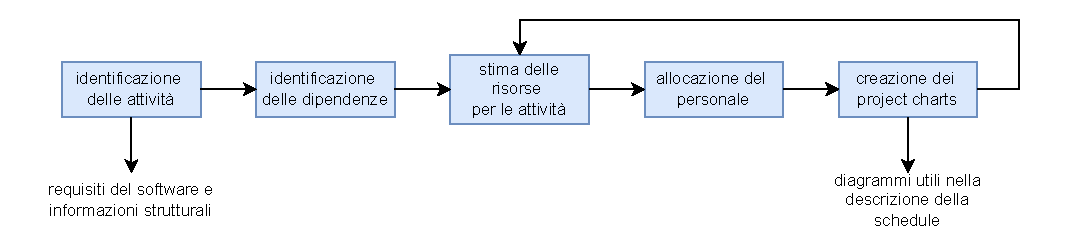
\includegraphics[width=1\textwidth ]{images/projectScheduling.pdf}
        \caption{Scheduling}
    \end{figure}\end{center}
\subsubsection{Problemi nello scheduling}\begin{itemize}
    \item Stimare la difficoltà del lavoro ed i costi di sviluppo è molto difficile 
    \item La produttività non è proporzionale al numero di persone coinvolte nel lavoro 
    \item L'aggiunta di personale a progetto già avviato può causare ritardi  
    \item Accade sempre l'inaspettato, bisogna considerare ogni evenienza nel planning
\end{itemize}
Esiste un annotazione grafica utile nella rappresentazione 
della schedule, mostra le diverse attività, il periodo in cui 
vanno terminate e le varie dipendenze fra esse, il diagramma a barre 
mostra le attività come risorse da disporre sull'asse dei 
tempi. Le "project activities" sono gli elementi di base del 
grafico, comprendono \begin{itemize}
    \item una durata sul calendario, di giorni o mesi 
    \item un carico di lavoro stimato, misurato in numero di 
    impiegati al giorno necessari
    \item una deadline per ogni attività che ne vincola 
    il completamento entro una certa data
    \item un punto specifico che descrive il terminamento di 
    un'attività, può essere un documento , una riunione o il completamento 
    di tutti i test
\end{itemize}
Una \textbf{milestone} non è altro che una "tappa 
fondamentale" durante lo svolgimento delle varie attività, può 
rappresentare un momento in cui si valuta la progressione del 
progetto.\acc 
Con \textbf{deliverables} si definiscono dei risultati ottenuti 
durante la lavorazione da presentare al cliente.








\redText{continua dalle slide "Ch23 Project planning" - pagina 30}
\end{document}